%package list
\documentclass{article}
\usepackage[top=3cm, bottom=3cm, outer=3cm, inner=3cm]{geometry}
\usepackage{multicol}
\usepackage{graphicx}
\usepackage{url}
%\usepackage{cite}
\usepackage{hyperref}
\usepackage{array}
%\usepackage{multicol}
\newcolumntype{x}[1]{>{\centering\arraybackslash\hspace{0pt}}p{#1}}
\usepackage{natbib}
\usepackage{pdfpages}
\usepackage{multirow}
\usepackage[normalem]{ulem}
\useunder{\uline}{\ul}{}
\usepackage{svg}
\usepackage{xcolor}
\usepackage{listings}
\lstdefinestyle{ascii-tree}{
    literate={├}{|}1 {─}{--}1 {└}{+}1 
  }
\lstset{basicstyle=\ttfamily,
  showstringspaces=false,
  commentstyle=\color{red},
  keywordstyle=\color{blue}
}
%\usepackage{booktabs}
\usepackage{caption}
\usepackage{subcaption}
\usepackage{float}
\usepackage{array}

\newcolumntype{M}[1]{>{\centering\arraybackslash}m{#1}}
\newcolumntype{N}{@{}m{0pt}@{}}


%%%%%%%%%%%%%%%%%%%%%%%%%%%%%%%%%%%%%%%%%%%%%%%%%%%%%%%%%%%%%%%%%%%%%%%%%%%%
%%%%%%%%%%%%%%%%%%%%%%%%%%%%%%%%%%%%%%%%%%%%%%%%%%%%%%%%%%%%%%%%%%%%%%%%%%%%
\newcommand{\itemEmail}{wroquequi@unsa.edu.pe}
\newcommand{\itemStudent}{William Isaias Roque Quispe}
\newcommand{\itemCourse}{Programación Web 2}
\newcommand{\itemSemester}{III}
\newcommand{\itemUniversity}{Universidad Nacional de San Agustín de Arequipa}
\newcommand{\itemFaculty}{Facultad de Ingeniería de Producción y Servicios}
\newcommand{\itemDepartment}{Departamento Académico de Ingeniería de Sistemas e Informática}
\newcommand{\itemSchool}{Escuela Profesional de Ingeniería de Sistemas}
\newcommand{\itemAcademic}{2023 - A}
\newcommand{\itemInput}{Del 29 junio 2023}
\newcommand{\itemOutput}{Al 14 de julio 2023}
\newcommand{\itemPracticeNumber}{07}
\newcommand{\itemTheme}{Relaciones de uno a muchos, muchos a muchos e impresión de pdf y emails}

%%%%%%%%%%%%%%%%%%%%%%%%%%%%%%%%%%%%%%%%%%%%%%%%%%%%%%%%%%%%%%%%%%%%%%%%%%%%
%%%%%%%%%%%%%%%%%%%%%%%%%%%%%%%%%%%%%%%%%%%%%%%%%%%%%%%%%%%%%%%%%%%%%%%%%%%%

\usepackage[english,spanish]{babel}
\usepackage[utf8]{inputenc}
\AtBeginDocument{\selectlanguage{spanish}}
\renewcommand{\figurename}{Figura}
\renewcommand{\refname}{Referencias}
\renewcommand{\tablename}{Tabla} %esto no funciona cuando se usa babel
\AtBeginDocument{%
	\renewcommand\tablename{Tabla}
}

\usepackage{fancyhdr}
\pagestyle{fancy}
\fancyhf{}
\setlength{\headheight}{30pt}
\renewcommand{\headrulewidth}{1pt}
\renewcommand{\footrulewidth}{1pt}
\fancyhead[L]{\raisebox{-0.2\height}{
\includegraphics[width=3cm]{img/logo_episunsa.png}}}
\fancyhead[C]{\fontsize{7}{7}\selectfont	\itemUniversity \\ \itemFaculty \\ \itemDepartment \\ \itemSchool \\ \textbf{\itemCourse}}
\fancyhead[R]{\raisebox{-0.2\height}{
\includegraphics[width=1.2cm]{img/logo_abet}}}
\fancyfoot[L]{Estudiante: William Roque Quispe}
\fancyfoot[C]{\itemCourse}
\fancyfoot[R]{Página \thepage}

% para el codigo fuente
\usepackage{listings}
\usepackage{color, colortbl}
\definecolor{dkgreen}{rgb}{0,0.6,0}
\definecolor{gray}{rgb}{0.5,0.5,0.5}
\definecolor{mauve}{rgb}{0.58,0,0.82}
\definecolor{codebackground}{rgb}{0.95, 0.95, 0.92}
\definecolor{tablebackground}{rgb}{0.8, 0, 0}

\lstset{frame=tb,
	language=bash,
	aboveskip=3mm,
	belowskip=3mm,
	showstringspaces=false,
	columns=flexible,
	basicstyle={\small\ttfamily},
	numbers=none,
	numberstyle=\tiny\color{gray},
	keywordstyle=\color{blue},
	commentstyle=\color{dkgreen},
	stringstyle=\color{mauve},
	breaklines=true,
	breakatwhitespace=true,
	tabsize=3,
	backgroundcolor= \color{codebackground},
}

\begin{document}
	\vspace*{10px}
	\begin{center}	
		\fontsize{17}{17} \textbf{ Informe de Laboratorio \itemPracticeNumber}
	\end{center}
	\centerline{\textbf{\Large Tema: \itemTheme}}
	%\vspace*{0.5cm}	

	\begin{flushright}
		\begin{tabular}{|M{2.5cm}|N|}
			\hline 
			\rowcolor{tablebackground}
			\color{white} \textbf{Nota}  \\
			\hline 
			     \\[30pt]
			\hline 			
		\end{tabular}
	\end{flushright}	

	\begin{table}[H]
		\begin{tabular}{|x{4.7cm}|x{4.8cm}|x{4.8cm}|}
			\hline 
			\rowcolor{tablebackground}
			\color{white} \textbf{Estudiante} & \color{white}\textbf{Escuela}  & \color{white}\textbf{Asignatura}   \\
			\hline 
			{\itemStudent \par \itemEmail} & \itemSchool & {\itemCourse \par Semestre: \itemSemester}     \\
			\hline 			
		\end{tabular}
	\end{table}		
	
	\begin{table}[H]
		\begin{tabular}{|x{4.7cm}|x{4.8cm}|x{4.8cm}|}
			\hline 
			\rowcolor{tablebackground}
			\color{white}\textbf{Laboratorio} & \color{white}\textbf{Tema}  & \color{white}\textbf{Duración}   \\
			\hline 
			\itemPracticeNumber & \itemTheme & 04 horas   \\
			\hline 
		\end{tabular}
	\end{table}
	
	\begin{table}[H]
		\begin{tabular}{|x{4.7cm}|x{4.8cm}|x{4.8cm}|}
			\hline 
			\rowcolor{tablebackground}
			\color{white}\textbf{Semestre académico} & \color{white}\textbf{Fecha de inicio}  & \color{white}\textbf{Fecha de entrega}   \\
			\hline 
			\itemAcademic & \itemInput &  \itemOutput  \\
			\hline 
		\end{tabular}
	\end{table}

        %Inicio
	\section{Tarea}
	\begin{itemize}
         \item Reproducir las actividades de los videos donde trabajamos:
         \begin{enumerate}
         \item Relación de uno a muchos
         \item Relación muchos a muchos
         \item Impresión de pdfs
         \item Envío de emails
         \end{enumerate}
         \end{itemize}
		
	\section{Equipos, materiales y temas utilizados}
	\begin{itemize}
		\item Sistema Operativo 
		\item GNU Vim.
		\item Python 3.11.3.
		\item Git
		\item Cuenta en GitHub con el correo institucional.
		\item Entorno virtual.
            \item Django 4.
            \item xhtml2pdf 0.2.11.
	\end{itemize}
	
	\section{URL de Repositorio Github}
	\begin{itemize}
		\item URL del Repositorio GitHub para clonar o recuperar.
		\item \url{https://github.com/WilliamIsaiasRoque/Lab07-Pweb2.git}
            \item URL del video subido en Flip.
            \item \url{https://flip.com/groups/14644257/topics/37115679/responses}
	\end{itemize}
	
	\section{Actividades}
	\subsection{Crear un directorio para el laboratorio}
	\begin{itemize}	
		\item En este directorio inicializaremos el git y agregaremos un primer commit para probar.
	\end{itemize}	

        \begin{lstlisting}[language=bash,caption={Creando directorio de trabajo y accediendo en él}][H]
		$ mkdir PWEB2lab/Lab07-Pweb2/
	\end{lstlisting}
	\begin{lstlisting}[language=bash,caption={Dirijiéndonos al directorio de trabajo}][H]
		$ cd PWEB2lab/Lab07-Pweb2/
	\end{lstlisting}	
	\begin{lstlisting}[language=bash,caption={Inicializando el repositorio Git y agregando remote add origin}][H]
		$ git init
		$ git remote add origin https://github.com/WilliamIsaiasRoque/Lab07-Pweb2.git
	\end{lstlisting}
        \begin{lstlisting}[language=bash,caption={Añadiendo un README.md como primer push}][H]
		$ echo "# Lab07-Pweb2" >> README.md
		$ git add README.md
		$ git commit -m "Initial commit"
		$ git push -u origin main
	\end{lstlisting}

        \subsection{Crear un entorno virtual en el directorio}
        \begin{lstlisting}[language=bash,caption={Creando el directorio django\_env y accediendo en esa carpeta}][H]
		$ virtualenv env
	\end{lstlisting}        	
        \begin{lstlisting}[language=bash,caption={Activando el entorno virtual con source}][H]
		$ source env/Scripts/activate
	\end{lstlisting} 
        \begin{lstlisting}[language=bash,caption={Instalando Django y xhtml2pdf (es una herramienta que convierte documentos XHTML a formato PDF.). Luego guardamos las versiones en un requirements.txt}][H]
        $ pip install Django
        $ pip install xhtml2pdf
        $ pip list
        Package    Version
        ---------- -------
        asgiref    3.7.2
        Django     4.2.2
        sqlparse   0.4.4
        tzdata     2023.3
        xhtml2pdf   0.2.11
        $ pip freeze > requirements.txt
	\end{lstlisting}
 
        \begin{lstlisting}[language=bash,caption={Creando tres proyectos Django para las tres actividades.}][H]
        $ django-admin startproject model_examples
        $ django-admin startproject pdfs_examples
        $ django-admin startproject emailexample
	\end{lstlisting}

        \subsection{Solución de ejercicios y commits}
        \begin{itemize}	
		\item Los commits más importantes aparecerán en esta sección, al final se mostrarán unas capturas con todos los commits.
		\item \textbf{PROYECTO model\_examples}
            \item Creamos una app con 'python manage.py startapp example'.
            \item Accedemos a los settings.py del proyecto y agregamos 'example' a INSTALLED APPS.
            \item Se agregaron distintos modelos al archivo 'models.py' los cuales hacen referencia a una tabla en la base de datos, se procede a explicar cada uno:
            \item El modelo Simple posee tres campos (text, number y url), con el método \_\_str\_\_ devuelve la URl almacenada.
            \item El modelo DateExample  tiene un campo llamado 'the\_date', que almacena una fecha y hora usando DateTimeField().
            \item El modelo NullExample tiene un área llamada col, encargada de almacenar texto con una longitud máxima de 10 caracteres.
            \item Para la relación uno a muchos se crearon los modelos Language y Framework, Language es capaz de guardar hasta 10 caracteres y Framework establece una relación de clave externa (ForeignKey) con el modelo Language.
            \item Para la relación muchos a muchos se adicionaron los modelos Movie y Character, Movie almacena texto hasta un límite de 10 caracteres y Character tiene un campo 'movies' que establece la relación 'ManyToManyField' con el modelo anterior. 
        \end{itemize}    
        \lstinputlisting[language=python, caption={model\_examples/example/models.py},numbers=left,]{src/model_examples/example/models.py}

        \begin{itemize}	
		\item Se ejecuta 'python manage.py makemigrations' para crear archivos de migración y después 'python manage.py migrate' para aplicar los cambios a la base de datos.
            \item En admin.py se registran todos los modelos creados anteriormente para que puedan ser utilizados correctamente.
            \item El resto de archivos no han sufrido cambios durante la elaboración de los modelos, por ello no se han agregado al informe.
        \end{itemize}
        \lstinputlisting[language=python, caption={model\_examples/example/admin.py},numbers=left,]{src/model_examples/example/admin.py}

        \begin{itemize}
            \item Se crearon diversas tablas usando los modelos a través de 'python manage.py shell'
            \item Para probar la relación uno a muchos, se creó la tabla example\_language con los elementos Python y Java, la tabla example\_framework posee los elementos Django, Flask, Bootle y Spring.
        \end{itemize}    
        \begin{figure}[ht]
        \centering
        \includegraphics[width=0.3\textwidth]{img/example\_language.png}
        \caption*{Tabla example\_character}
        \end{figure}
        \begin{figure}[ht]
        \centering
        \includegraphics[width=0.3\textwidth]{img/example\_framework.png}
        \caption*{Tabla example\_character}
        \end{figure}

        \begin{itemize}
            \item Se realizaron consultas (query) para recoletar los datos de las tablas. Para ello se volvió a acceder a 'Python manage.py shell'.
        \end{itemize}
        \begin{lstlisting}[language=bash,caption={Query One To Many}][H]
            from example.models import Language, Framework
            Framework.objects.all()
            Framework.objects.filter(language__name='Python')
            Framework.objects.filter(language__name='Java')
            Framework.objects.filter(language__name__startswith='Py')
            Framework.objects.filter(language__name__startswith='Ja')
            Language.objects.filter(framework__name='Spring')
            Language.objects.filter(framework__name='Django')
	\end{lstlisting}

        \begin{itemize}
            \item Para probar la relación muchos a muchos, se creó la tabla example\_character con los elementos Captain America y Thor, la tabla example\_movie contiene un listado de películas (Avengers, Civil War, Thor: Dark World y Winter Soldier). 
            \item La tabla example\_character\_movies demuestra que un actor puede estar asociado a varias películas y viceversa.
        \end{itemize}    
        \begin{figure}[H]
        \centering
        \includegraphics[width=0.3\textwidth]{img/example\_character.png}
        \caption*{Tabla example\_character}
        \end{figure}
        \begin{figure}[ht]
        \centering
        \includegraphics[width=0.3\textwidth]{img/example\_movie.png}
        \caption*{Tabla example\_movie}
        \end{figure}
        \begin{figure}[ht]
        \centering
        \includegraphics[width=0.3\textwidth]{img/example\_character\_movies.png}
        \caption*{Tabla example\_character\_movies}
        \end{figure}
        
        \begin{itemize}
            \item Se realizaron otras consultas (query) para recoletar los datos de las tablas mediante shell.
        \end{itemize}
        \begin{lstlisting}[language=bash,caption={Many To Many Query}][H]
            from example.models import Character, Movie
            Character.objects.filter(movies__name='Civil War')
            Character.objects.filter(movies__name='Avengers')
            Movie.objects.filter(character__name='Captain America')
            Movie.objects.filter(character__name='Thor')
            captain_america = Character.objects.get(name='Captain America')
            captain_america
            captain_america.movies.all()
            avengers = Movie.objects.get(name='Avengers')
            avengers
            avengers.character_set.all()
	\end{lstlisting}

        \begin{itemize}	
		\item \textbf{PROYECTO pdfs\_examples}
            \item Para este proyecto no será necesario crear una aplicación extra ya que se agregarán los archivos requeridos directamente en la carpeta base.
            \item Se agrega 'utils.py' para convertir un archivo HTML en un archivo PDF utilizando la biblioteca xhtml2pdf. Si no hay errores durante la conversión del HTML a PDF, se devuelve un objeto HttpResponse que contiene los datos del PDF generado, con el tipo de contenido establecido como 'application/pdf'.
        \end{itemize} 
        \lstinputlisting[language=python, caption={pdfs\_examples/utils.py},numbers=left,]{src/pdfs_examples/pdfs_examples/utils.py}  
        \begin{itemize}
            \item Después se ha modificado la ruta de TEMPLATES DIRS en settings.py para que utilice la carpeta templates que se creará pronto.
            \item Se debe agregar el archivo views.py el cual se encargará de generar un archivo PDF, cuando se accede a la vista a través de una solicitud GET, se carga la plantilla HTML, se renderiza con los datos del contexto y termina generándose el PDF. Si se ha creado correctamente, devuelve una respuesta HTTP adjunta según los parámetros de la solicitud GET. En caso contrario, retorna una respuesta indicando que no se encontró el elemento.
            \item Para urls.py se debe agregar 'pdf/' para generar y devolver un archivo PDF utilizando la vista GeneratePdf. 
        \end{itemize}
        \lstinputlisting[language=python, caption={pdfs\_examples/views.py},numbers=left,]{src/pdfs_examples/pdfs_examples/views.py} 
        \lstinputlisting[language=python, caption={pdfs\_examples/urls.py},numbers=left,]{src/pdfs_examples/pdfs_examples/urls.py} 

        \begin{itemize}
            \item Es importante crear la carpeta templates, acceder y crear otra carpeta llamada pdf, dentro de esta nueva carpeta se inicializará un index.html, el cual tiene un estilo y estructura predeterminada para mostrar información de una factura. Los valores de invoice\_id, customer\_name, amount y today se insertarán en los lugares correspondientes cuando se renderice la plantilla con datos específicos.
        \end{itemize}
        \lstinputlisting[language=html, caption={pdfs\_examples/templates/pdf/invoice.html},numbers=left,]{src/pdfs_examples/templates/pdf/invoice.html} 
        \begin{figure}[H]
        \centering
        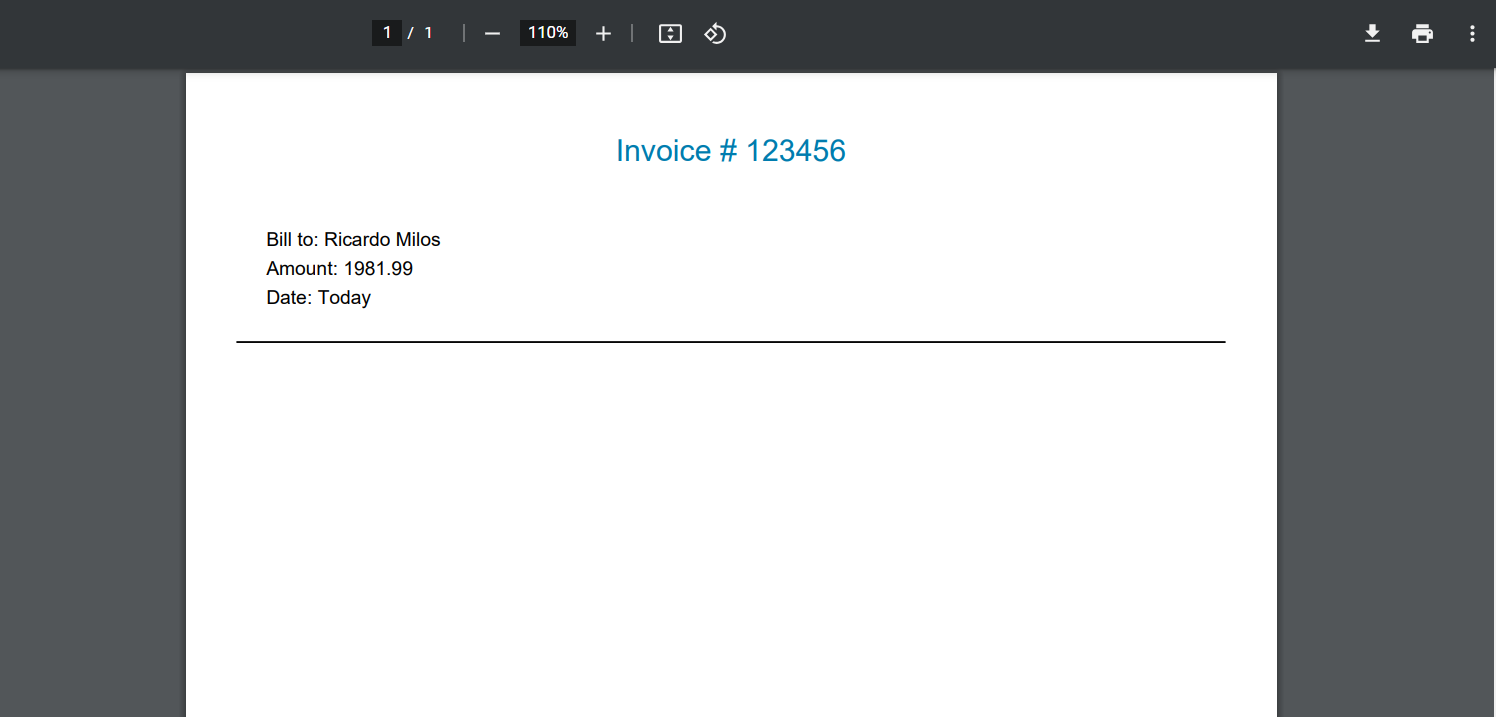
\includegraphics[width=0.8\textwidth]{img/pdfexample.png}
        \caption*{Ejecución del servidor}
        \end{figure}
        \vspace{0.5cm} %espacio de separacion
        \begin{itemize}	
		\item \textbf{PROYECTO emailexample}
            \item Primero se inicia una app con 'python manage.py startapp send', después se accede a settings.py para agregar a 'send' en INSTALLED APPS.
            \item Luego se agregó el archivo urls.py dentro de la carpeta send.
        \end{itemize} 
        \lstinputlisting[language=python, caption={emailexample/send/urls.py},numbers=left,]{src/emailexample/send/urls.py} 
        \begin{itemize}	
            \item Se procede a modificar el urls.py del proyecto (es distinto al de send).
        \end{itemize}
        \lstinputlisting[language=python, caption={emailexample/emailexample/urls.py},numbers=left,]{src/emailexample/emailexample/urls.py} 

        \begin{itemize}	
            \item Dentro de la carpeta send se crea un directorio llamado templates, se accede a él y se crea otro directorio llamado send al cual debemos acceder nuevamente, para finalmente crear un index.html el cual tiene de título 'Sent!' y muestra en pantalla un mensaje confirmando el envío del email.
        \end{itemize}
        \lstinputlisting[language=html, caption={emailexample/send/templates/send/index.html},numbers=left,]{src/emailexample/send/templates/send/index.html} 
        \begin{itemize}	
            \item En settings.py se agrega la información necesaria para enviar correos electrónicos utilizando el servidor SMTP de Gmail. Se especifica el servidor, el puerto, la dirección de correo electrónico y la contraseña del remitente. También se establece si se utilizará TLS para la conexión segura.
        \end{itemize}
        \begin{figure}[H]
        \centering
        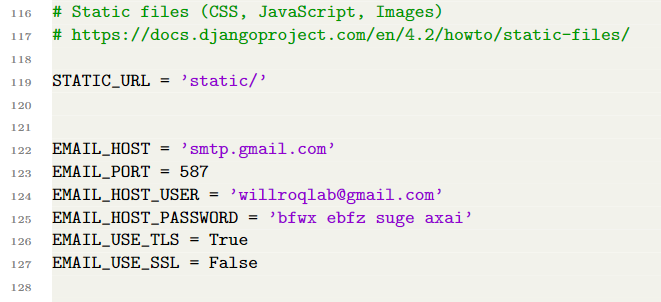
\includegraphics[width=0.6\textwidth]{img/settings.png}
        \caption*{Configuración de emails}
        \end{figure}
        \begin{itemize}	
            \item En views.py se define una vista que envía un correo electrónico utilizando la función 'send\_mail' y luego muestra una página HTML mediante la función render. El correo electrónico tiene un asunto, un cuerpo y se envía desde la dirección de correo electrónico especificada al destinatario indicado. Después de enviar el correo electrónico, se muestra una página HTML al usuario.
        \end{itemize}
        \lstinputlisting[language=python, caption={emailexample/send/views.py},numbers=left,]{src/emailexample/send/views.py} 

        \begin{figure}[H]
        \centering
        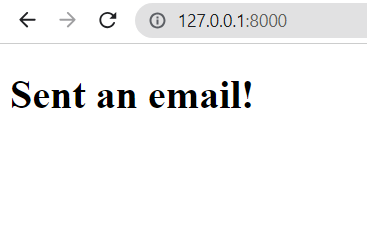
\includegraphics[width=0.6\textwidth]{img/sentemail.png}
        \caption*{Ejecución del servidor}
        \end{figure}
        \vspace{1cm}
        \begin{figure}[H]
        \centering
        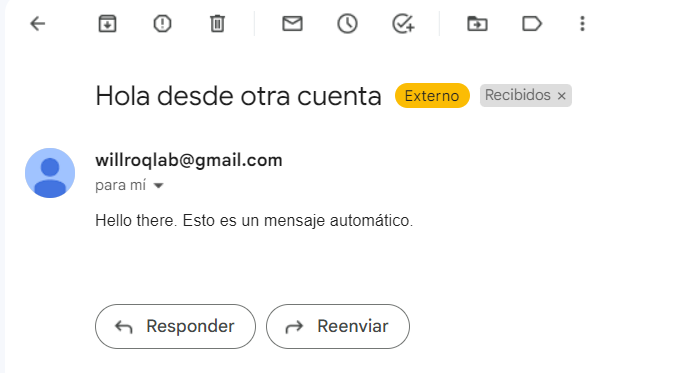
\includegraphics[width=0.6\textwidth]{img/viewemail.png}
        \caption*{Mensaje recibido en la bandeja de entrada}
        \end{figure}
        \vspace{2cm}
        \begin{itemize}	
		\item A continuación una captura de todos los commits realizados en el repositorio GitHub:
        \end{itemize}
        \vspace{0.5cm}
        \begin{figure}[H]
        \centering
        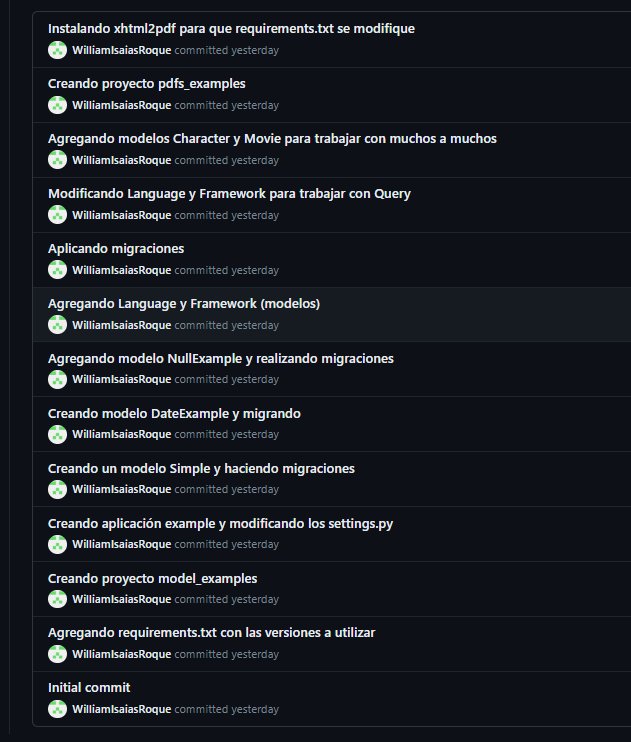
\includegraphics[width=0.4\textwidth]{img/commits01.png}
        \caption*{Primera parte de los commits}
        \end{figure}
        \begin{figure}[H]
        \centering
        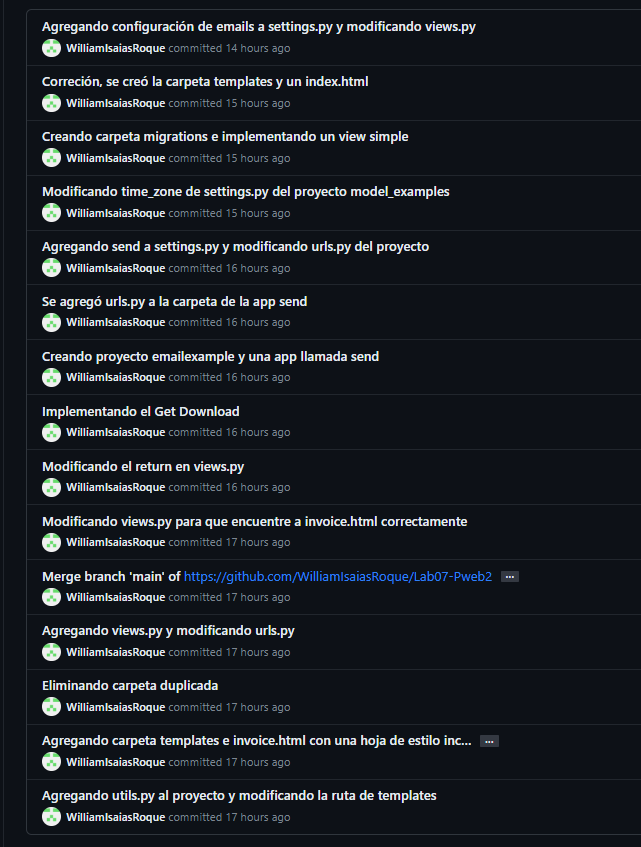
\includegraphics[width=0.4\textwidth]{img/commits02.png}
        \caption*{Segunda parte de los commits}
        \end{figure}
        \vspace{0.5cm}
        \section{Conclusiones}
	\begin{itemize}			
		\item Django ofrece un enfoque sencillo para gestionar relaciones One-to-Many entre modelos. Con la utilización de campos ForeignKey o OneToManyField, se facilita la creación y manipulación de relaciones entre tablas.
            \item Django se encarga automáticamente de la creación de tablas intermedias para almacenar los vínculos entre los objetos relacionados de muchos a muchos con ManyToManyField.
            \item Con el uso de bibliotecas como ReportLab, xhtml2pdf o WeasyPrint, se pueden generar archivos PDF dinámicamente a partir de plantillas o datos y servirlos como una respuesta HTTP. 
            \item A través del módulo django.core.mail, es posible configurar los parámetros de un servidor SMTP, establecer los destinatarios, asunto, cuerpo y adjuntos de los correos electrónicos y enviar emails.
	\end{itemize}

        \section{Referencias}
	\begin{itemize}		
            \item \url{https://www.pythontutorial.net/django-tutorial/django-one-to-many/}
		\item \url{https://docs.djangoproject.com/en/4.2/topics/db/examples/many_to_many/}
            \item \url{https://www.codingforentrepreneurs.com/blog/html-template-to-pdf-in-django/}
            \item \url{https://docs.djangoproject.com/en/4.2/topics/email/}
	\end{itemize}        
 \end{document}